\section{Instruction Language} 

\subsection{Addressing Modes}

  Registers being 8 bytes mean that we can store memory addresses, and if we can store memory addresses, we can access memory, i.e. the values at those memory addresses. There are 4 ways to do this, called \textbf{addressing modes}: immediate, normal, displacement, and indexed. When we parse an instruction, its operands are either 
  \begin{enumerate}
    \item Constant (literal) values 
    \item Registers 
    \item Memory forms
  \end{enumerate}

  \begin{definition}[Immediate Addressing]
    Immediate addressing is when the operand is a constant value, used with a \$ sign. 
    \begin{equation}
      \texttt{\$val}
    \end{equation}
  \end{definition}

  \begin{definition}[Normal Addressing]
    Normal addressing is when the operand is a register, used with a \% sign and the following syntax. The parentheses are used to dereference the memory address like dereferencing a pointer in C. 
    \begin{equation}
      \texttt{(R) = Mem[Reg[R]]}
    \end{equation}
    where \texttt{R} is the register name, \texttt{Reg[R]} is the value in the register, and \texttt{Mem[Reg[R]]} is the value in the memory address pointed to by the register. 
  \end{definition}

  \begin{definition}[Displacement Addressing]
    When we have a memory address stored in a register, we can add an offset to it to access a different memory address. 
    \begin{equation}
      \texttt{D(R) = Mem[Reg[R] + D]}
    \end{equation}
    where \texttt{R} is the register name and \texttt{D} is a constant displacement that specifies offset. 
  \end{definition}

  \begin{definition}[Indexed Addressing]
    Indexed addressing gives us more flexibility, allowing us to multiply the value in the register by a constant and add it to the value in another register. The general formula is shown as the top, but there are special cases: 
    \begin{align*}
      \texttt{D(Rb, Ri, S)} && = \texttt{Mem[Reg[Rb] + S*Reg[Ri] + D]} \\ 
      \texttt{D(Rb, Ri)} && = \texttt{Mem[Reg[Rb] + Reg[Ri] + D]} \\
      \texttt{(Rb, Ri, S)} && = \texttt{Mem[Reg[Rb] + S*Reg[Ri]]} \\ 
      \texttt{(Rb, Ri)} && = \texttt{Mem[Reg[Rb] + Reg[Ri]]} \\
      \texttt{(, Ri, S)} && = \texttt{Mem[S*Reg[Ri]]} 
    \end{align*}
    where \texttt{D} is a constant displacement of 1, 2, or 4 bytes, \texttt{Rb} is the base register (can be any of 8 integer registers), \texttt{Ri} is the index register (can be any register except \texttt{rsp}), and \texttt{S} is the scale factor (1, 2, 4, or 8). 
  \end{definition}

\subsection{Instructions}

    Now let's talk about how functions work on a deeper level. When we write a command, like \texttt{int x = 4}, we are manually looking for an address (in the stack, global, or heap) and rewriting the bits that are at that address. Functions are just an automated way to do this, and all these modifications and computations are done by the CPU. 

    \begin{definition}[Central Processing Unit]
      The CPU is responsible for taking instructions (data) from memory and executing them. 
      \begin{enumerate} 
        \item The CPU is composed of \textbf{registers} (different from the cache), which are small, fast storage locations. These registers can either be \textbf{general purpose} (can be used with most instructions) or \textbf{special purpose} (can be accessed through special instructions, or have special meanings/uses, or are simply faster when used in a specific way).
        \item The CPU also has an \textbf{arithmetic unit} and \textbf{logic unit}, which is responsible for performing arithmetic and logical operations. 
        \item The CPU also has a \textbf{control unit}, which is responsible for fetching instructions from memory through the \textbf{databus}, which is literally a wire connecting the CPU and RAM, and executing them. 
      \end{enumerate}
      It executes instructions from memory one at a time and executes them, known as the \textbf{fetch-execute cycle}. It consists of 4 main operations. 
      \begin{enumerate} 
        \item \textbf{Fetch}: The \textbf{program counter}, which holds the memory address of the next instruction to be executed, tells the control unit to fetch the instruction from memory through the databus. 
        \item \textbf{Decode}: The fetched data is passed to the \textbf{instruction decoder}, which figures out what the instruction is and what it does and stores them in the registers.
        \item \textbf{Execute}: The arithmetic and logic unit then carries out these operations. 
        \item \textbf{Store}: Then it puts the results back on the databus, and stores them back into memory.
      \end{enumerate} 
      The CPU's \textbf{clock cycle} is the time it takes for the CPU to execute one instruction. More specifically, the clock cycle refers to a single oscillation of the clock signal that synchronizes the operations of the processor and the memory (e.g. fetch, decode, execute, store), and decent computers have clock cycles of at least $2.60$GHz (2.6 billion clock cycles per second). 
    \end{definition}

    Therefore, in order to actually do computations on the data stored in the memory, the CPU must first fetch the data, perform the computations, and then store the results back into memory. This can be done in two ways.

    \begin{enumerate}
      \item Load and Store Operations: CPUs use load instructions to move data from memory to registers (where operations can be performed more quickly) and store instructions to move the modified data back into memory.
      \item If the data is too big to fit into the registers, the CPU will use the \textbf{cache} to store the data, and in worse cases, the actual memory itself. Compilers optimize code by maximizing the use of registers for operations to minimize slow memory access. This is why you often see assembly code doing a lot in registers.
    \end{enumerate}

    To clarify, let us compare registers and memory. Memory is addressed by an unsigned integer while registers have names like \texttt{\%rsi}. Memory is much bigger at several GB, while the total register space is much smaller at around 128 bytes (may differ depending on the architecture). The memory is much slower than registers, which is usually on a sub-nanosecond timescale. The memory is dynamic and can grow as needed while the registers are static and cannot grow.

    The specific structure/architecture of the CPU is determined by the instruction set architecture (ISA), which can be thought of as a subset of the general computer architecture. 

    \begin{definition}[Instruction Set Architecture]
      The \textbf{ISA} or just \textbf{architecture} of a CPU is a high level description of what it can do. Some differences are listed here: 
      \begin{enumerate} 
        \item What instructions it can execute. 
        \item The instruction length and decoding, along with its complexity. 
        \item The performance vs power efficiency. 
      \end{enumerate}
      ISAs can be classified into two types. 
      \begin{enumerate} 
        \item The \textbf{complex instruction set computer} (CISC) is characterized by a large set of complex instructions, which can execute a variety of low-level operations. This approach aims to reduce the number of instructions per program, attempting to achieve higher efficiency by performing more operations with fewer instructions.
        \item The \textbf{reduced instruction set computer} (RISC) emphasizes simplicity and efficiency with a smaller number of instructions that are generally simpler and more uniform in size and format. This approach facilitates faster instruction execution and easier pipelining, with the philosophy that simpler instructions can provide greater performance when optimized.
      \end{enumerate}
    \end{definition}

  \subsection{Instructions} 

      Now that we've gotten a sense of what these registers are and some commonalities between them, let's do some operations on them with instructions. 

      \begin{definition}[Instruction]
        An instruction is a single line of assembly code. It consists of some instruction followed by its (one or more) operands. The instruction is a mnemonic for a machine language operation (e.g. \texttt{mov}, \texttt{add}, \texttt{sub}, \texttt{jmp}, etc.). The \textbf{size specifier} can be appended to this instruction mnemonic to specify the size of the operands. 
        \begin{enumerate} 
          \item \textbf{b} (byte) for 1 byte 
          \item \textbf{w} (word) for 2 bytes
          \item \textbf{l} (long) for 4 bytes 
          \item \textbf{q} (quad word) for 8 bytes
        \end{enumerate}
        Note that due to backwards compatibility, word means 2 bytes in instruction names. Furthermore, the maximum size is 8 bytes since that is the size of each register in x86\_64. An operand can be of 3 types, determined by their \textbf{mode of access}:
        \begin{enumerate} 
          \item \textbf{Immediate addressing} is denoted with a \texttt{\$} sign, e.g. a constant integer data \texttt{\$1}. 
          \item \textbf{Register addressing} is denoted with a \texttt{\%} sign with the following register name, e.g. \texttt{\%rax}.
          \item \textbf{Memory addressing} is denoted with the hexadecimal address in memory, e.g. \texttt{0x034AB}.
        \end{enumerate}
      \end{definition}

      Like higher level programming languages, we can perform operations, do comparisons, and jump to different parts of the code. Instructions can be generally categorized into three types: 
      \begin{enumerate} 
        \item \textbf{Data Movement}: These instructions move data between memory and registers or between the registery and registery. Memory to memory transfer cannot be done with a single instruction. 
          \begin{lstlisting} 
            %reg = Mem[address]     # load data from memory into register
            Mem[address] = %reg     # store register data into memory
          \end{lstlisting}
        \item \textbf{Arithmetic Operation}: Perform arithmetic operation on register or memory data. 
          \begin{lstlisting} 
            %reg = %reg + Mem[address]     # add memory data to register
            %reg = %reg - Mem[address]     # subtract memory data from register
            %reg = %reg * Mem[address]     # multiply memory data to register
            %reg = %reg / Mem[address]     # divide memory data from register
          \end{lstlisting}
        \item \textbf{Control Flow}: What instruction to execute next both unconditional and conditional (if statements) ones. With if statements, loops can then be defined. 
          \begin{lstlisting} 
            jmp label     # jump to label
            je label      # jump to label if equal
            jne label     # jump to label if not equal
            jg label      # jump to label if greater
            jl label      # jump to label if less
            call label    # call a function
            ret           # return from a function
          \end{lstlisting}
      \end{enumerate}

      Now unlike compiled languages, which are translated into machine code by a compiler, assembly code is translated into machine code through a two-step process. First, we \textbf{assemble} the assembly code into an \textbf{object file} by an \textbf{assembler}, and then we \textbf{link} the object file into an executable by a \textbf{linker}. Some common assemblers are \textbf{NASM} (Netwide Assembler) and \textbf{GAS/AS} (GNU Assembler), and common linkers are \textbf{ld} (GNU Linker) and \textbf{lld} (LLVM Linker), both installable with \textbf{sudo pacman -S nasm ld}. 

    \subsubsection{Moving and Arithmetic} 

      Again, it is more important to have a general feel of what instructions every assembly language should  and get the ideas down rather than the syntax. We list them here, beginning with simply moving. 


      \begin{definition}[Moving]
        
      \end{definition}

      Next we want to have some sort of arithmetic to do calculations and to compare values. 

      \begin{definition}[Arithmetic Operations]
        
      \end{definition}

    \subsubsection{Conditionals}

      \begin{definition}[Conditionals]
        
      \end{definition}

    \subsubsection{Control Transfer on Stack}

      These are really the three basic functions needed to do anything in assembly, but let's talk about an important implementation called the \textbf{control transfer}. Say that you want to compute a function. 
      \begin{enumerate}
        \item Then we must retrieve the data from the memory. 
        \item We must load it into our registers in the CPU and perform some computation. 
        \item Then we must store the data back into memory. 
      \end{enumerate}

      Let’s begin with a refresher on how the call stack is managed. Recall that \texttt{\%rsp} is the stack pointer and always points to the top of the stack. The register \texttt{\%rbp} represents the base pointer (also known as the frame pointer) and points to the base of the current stack frame. The stack frame (also known as the activation frame or the activation record) refers to the portion of the stack allocated to a single function call. The currently executing function is always at the top of the stack, and its stack frame is referred to as the active frame. The active frame is bounded by the stack pointer (at the top of stack) and the frame pointer (at the bottom of the frame). The activation record typically holds local variables for a function.

      \begin{figure}[H]
        \centering 
        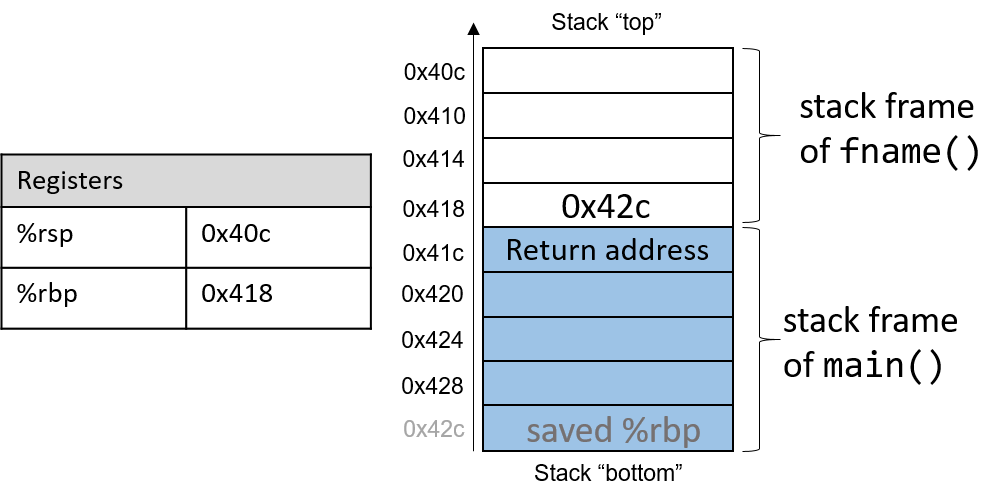
\includegraphics[scale=0.6]{img/stackFrame.png}
        \caption{The current active frame belongs to the callee function (fname). The memory between the stack pointer and the frame pointer is used for local variables. The stack pointer moves as local values are pushed and popped from the stack. In contrast, the frame pointer remains relatively constant, pointing to the beginning (the bottom) of the current stack frame. As a result, compilers like GCC commonly reference values on the stack relative to the frame pointer. In Figure 1, the active frame is bounded below by the base pointer of fname, which is stack address 0x418. The value stored at address 0x418 is the "saved" \texttt{\%rbp} value (0x42c), which itself is an address that indicates the bottom of the activation frame for the main function. The top of the activation frame of main is bounded by the return address, which indicates where in the main function program execution resumes once the callee function fname finishes executing. }
        \label{fig:stack_frame_management}
      \end{figure}


      Once we have done this we are really done. Formally, this is called Turing complete (?). 

      \begin{definition}[Control Transfers]
        We list some. 
        \begin{enumerate}
          \item Push 
          \item Pop 
          \item Call to call a function 
          \item Return to return from a function 
          \item Continue 
          \item Get out of stack with leave.  
        \end{enumerate}
      \end{definition}

      \begin{example}[Control Transfer Example]
        We show this with a minimal example with psuedocode. 
      \end{example}

    \subsubsection{Multiple Functions}

      Now what happens if there are multiple functions calling each other? Take a look at the following example with two functions. 

      \begin{example}[Multiple Functions Example]
        
      \end{example}

      There is a bit of a concern here from the previous example. The main function had two functions that returned two values. As the subfunction stack frame is removed from the stack, the return value is stored in the \texttt{\%rax} register. If another function is called right after, then the return value of the second function will overwrite that of the previous one. This was not a problem in the previous example since the return value of the \texttt{assign} function was not used. However, if it was, then the return value of the \texttt{adder} function would have overwritten it. This is known as register saving. 
      \begin{enumerate}
        \item For \textbf{caller-saved registers}, the caller function is responsible for saving the value of the register before calling a function and restoring it after the function returns. The caller should save values in its stack frame before calling the callee function, e.g. by pushing all the return values of each callee in the caller stack frame. Then it will restore values after the call. 

        \begin{center}
          \textit{Therefore, if we have a set of registers $\{\texttt{\%reg}\}$, the caller must take everything and push them in the caller stack frame. Then it will restore them after the call.}
        \end{center}

        \item For \textbf{callee-saved registers}, it is the callee's responsibility to save any data in these registers before using the registers. 

          \begin{center} 
            \textit{Therefore, if we have a set of registers $\{\texttt{\%reg}\}$, then inside the callee stack frame, the callee must take everything and push them in the callee stack frame. Once it computes the final return value, then it will restore all the saved register values from the callee stack frame back into the registers for the caller to use.}
          \end{center}
      \end{enumerate}

      Ideally, we want \textit{one} calling convention to simply separate implementation details between caller and callee. In general, however, neither is best. If the caller isn't using a register, then caller-save is better, and if callee doesn't need a register, then callee-save is better. If we do need to save, then callee save generally makes smaller programs, so we compromise and use a combination of both caller-save and callee-save. 



